

%% bare_conf.tex
%% V1.3
%% 2007/01/11
%% by Michael Shell
%% See:
%% http://www.michaelshell.org/
%% for current contact information.

\documentclass[conference]{IEEEtran}


\usepackage{graphicx}
\usepackage{float}
\usepackage{listings}


% *** GRAPHICS RELATED PACKAGES ***
%
\ifCLASSINFOpdf

\else

\fi

\hyphenation{op-tical net-works semi-conduc-tor}


\begin{document}
%
% paper title
% can use linebreaks \\ within to get better formatting as desired
\title{Report of Invidual project T1 - StandingSick}


% author names and affiliations
% use a multiple column layout for up to three different
% affiliations
\author{\IEEEauthorblockN{Lukasz Swiderski}
\IEEEauthorblockA{Universidade da Beira Interior\\
Covilha, Portugal\\
a36724\\
web: http://www.swiderski.xyz\\
email: lukasz@swiderski.xyz}}



\maketitle


\IEEEpeerreviewmaketitle



\section{Introduction}
% no \IEEEPARstart
StandingSick is project of application that allow user who
is waiting in queue to the doctor in hospital, save the time
of future medical examination, by fill the survey of his actual state.


\subsection{Goals}
The main goal of the project is ask a user for bunch of qeuestions
in the easiest way. Show the report for the doctor, send
the report by e-email to him, or save it on external storage. 
Look into the history of past answers. And modify the questions 
and answers by the administrator.

\subsection{Structure of the report}
The report was divided on 2 parts. First is describing the architecture
and design of application. When the second one is describing the 
implementation of the project.


\section{Interface Design and Application Architecture}

First topic to touch is the architecture of the application and
the structure of the database. Next topic are main modules of the 
application. Finaly the last part of the secion is design of interface and will 
be showed the screens of aplications and the used xml solutions to get it.

\subsection{Application Architecture}

\paragraph{} Each screen of the aplication is a separate Activity. To moving between the 
activities are used intentions. Content what is showing by the activity is loaded
with the activity, only the activity with questions is different because there 
content is changing after answer. The list of Activities: MainActivity, AdminActivity, 
AdminQuestionActivity, DatabaseActivity, PasswordActivity, ResultActivity, SurveyActivity.

\paragraph{} To store data is used SQLite database. Every action is executing the SQL query.

\subsection{Entity Relationship Model}

In the project are used 4 tables: Questions, Answers, Sessions and UserAnswers. 
Questions table got 2 columns: Id and Content, where the first one is primary key 
and second one contains the questions. Table Answers got 3 columns: Id, Content 
and QId, where the Id is primary key, Content contains the answer and QId is foreign key to table 
Questions to specific question with the answer is connected. Table Sessions got 2 colums Id and Date 
and it is storing the information when the user started answering the questions.
The last table UserAnswers got 6 columns: Id, SessionID, QId, AId, Question and Answer. 
In that table are stored information about the what answer what selected in wchich question and by the
foreign key to session when the answer was given.

\subsection{Program Description}

The application was divided to 3 modules: Survey, History and Admin Panel. 
\paragraph{Survey} The first one is showing the questions with possible answer to the user, one per page. Entrance to the survey is automatically creates a new session. When user 
already select the answer, he need to confirm it by click to the next button and the new question will 
appear. Until he did not click to the next button he can change the answer. If user want to skip the 
question he can do it by pressing the next button without select answer. The question will be skipped in report too.
After all questions user is moved to result activity where report is shown and user is asked for: saving the report 
in txt format at external storage, send the email with the report, or back to the menu. After selecting the save option, 
user will receive the short toast message with localization of the file. 
\paragraph{History} In this module user got lists with all selected answer in the past, divided by the sessions and sorted from the newest to the oldest. After choose the session there will be show a report from this time with every selected anser, and user will can save it as txt or send it to the doctor again.
\paragraph{Admin Panel} In the last module user is asked for the password (admin123). If he put correct, he will be moved to the list of the question. There he can select existed question or create new one. After choose he is moved to activity with edit options for the selected question. Delete or change content of the question, add, change or remove answers.


\subsection{Interface}


\begin{figure}[p!]
  \centering
      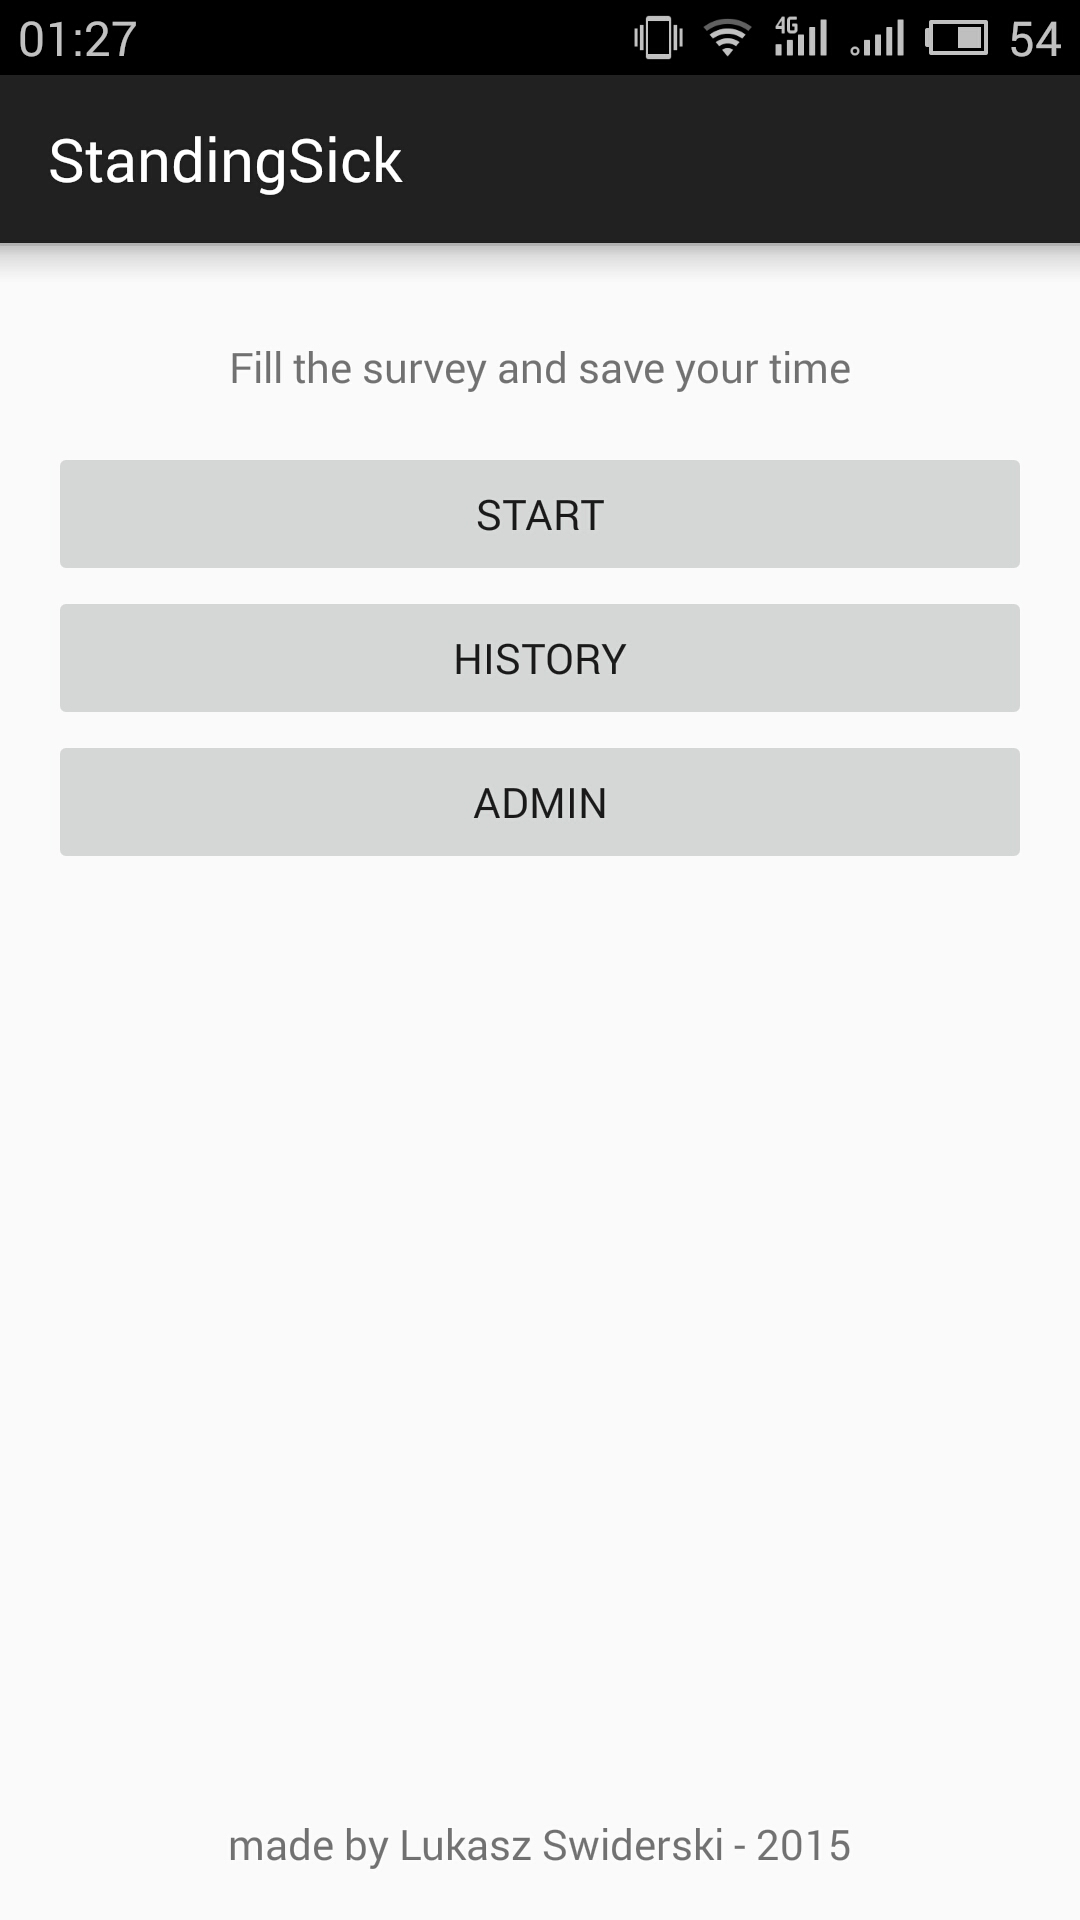
\includegraphics[width=2.0in]{./../img/main_menu.jpg}
  \caption{main menu}
  \label{main-menu-ss}
\end{figure}

\begin{figure}[p!]
  \centering
      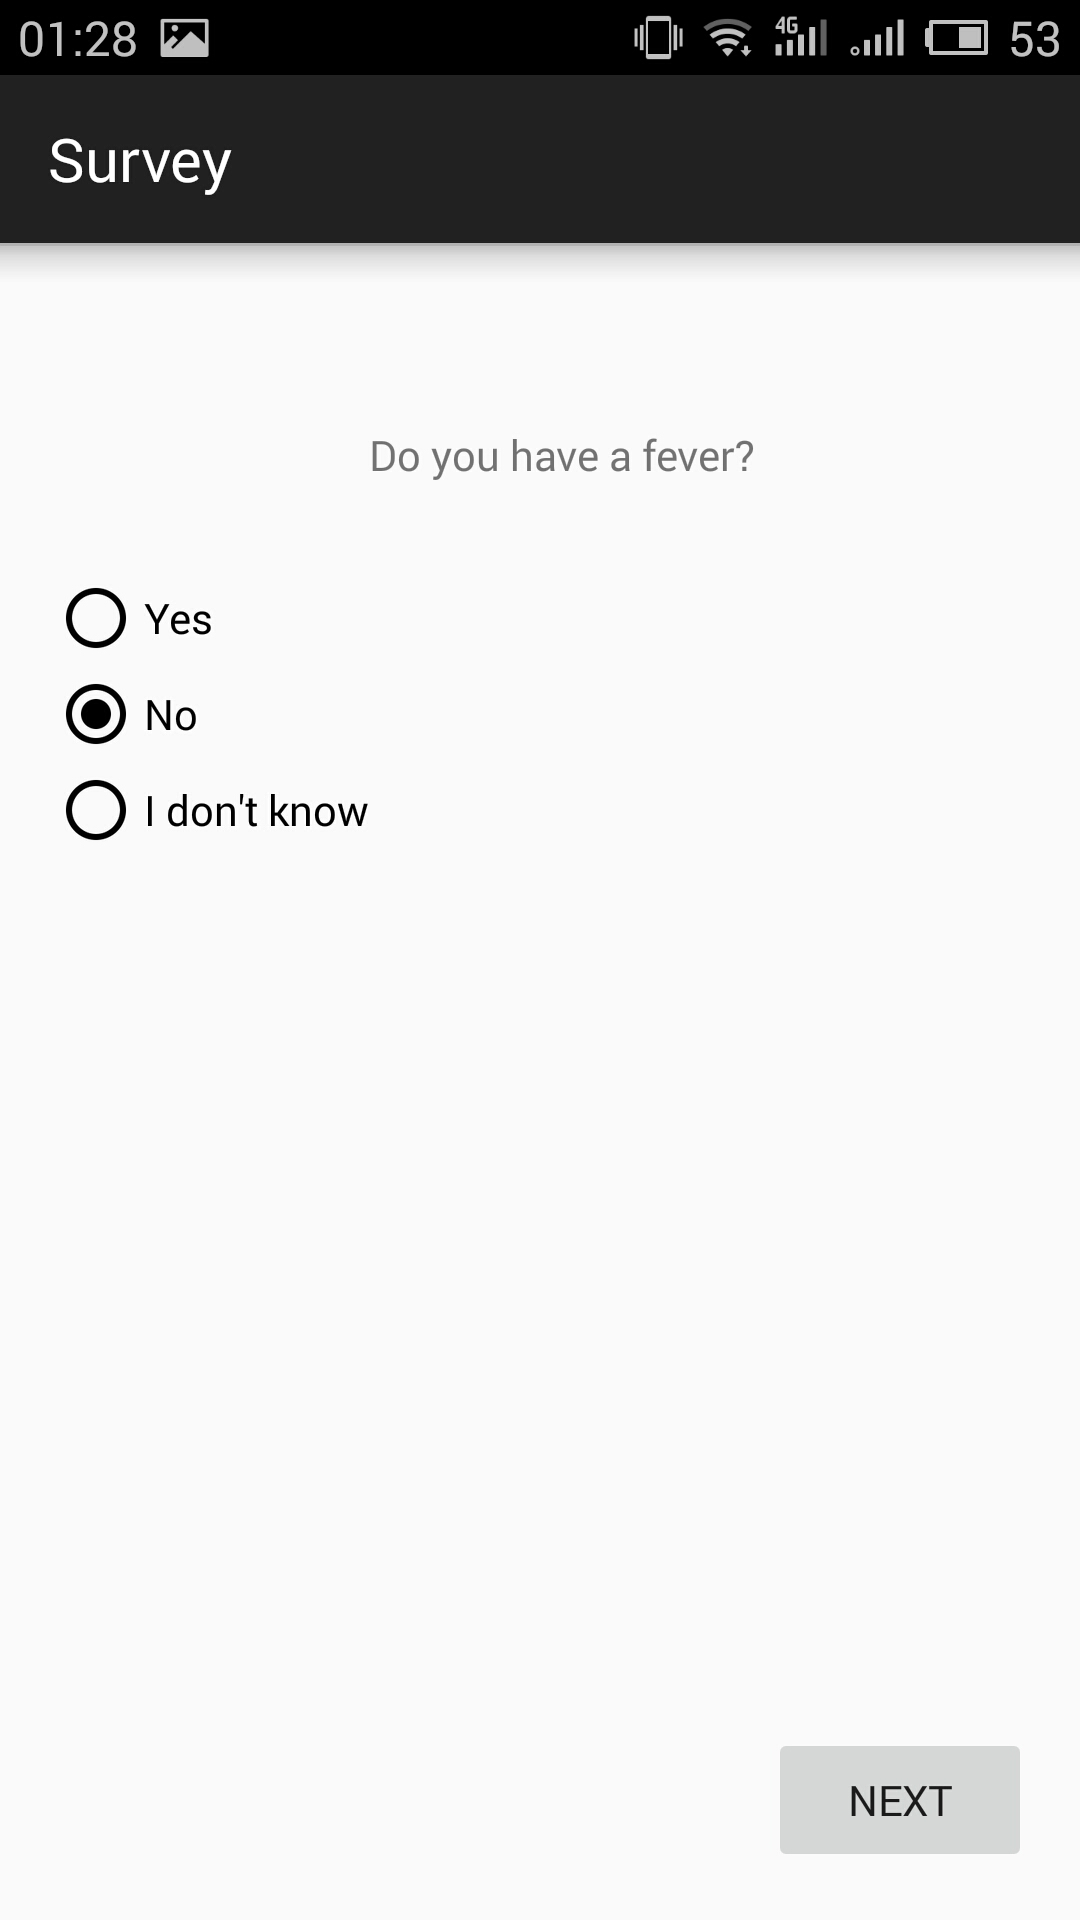
\includegraphics[width=2.0in]{./../img/survey.jpg}
  \caption{Survey Activity}
  \label{poll-ss}
\end{figure}

\begin{figure}[p!]
  \centering
      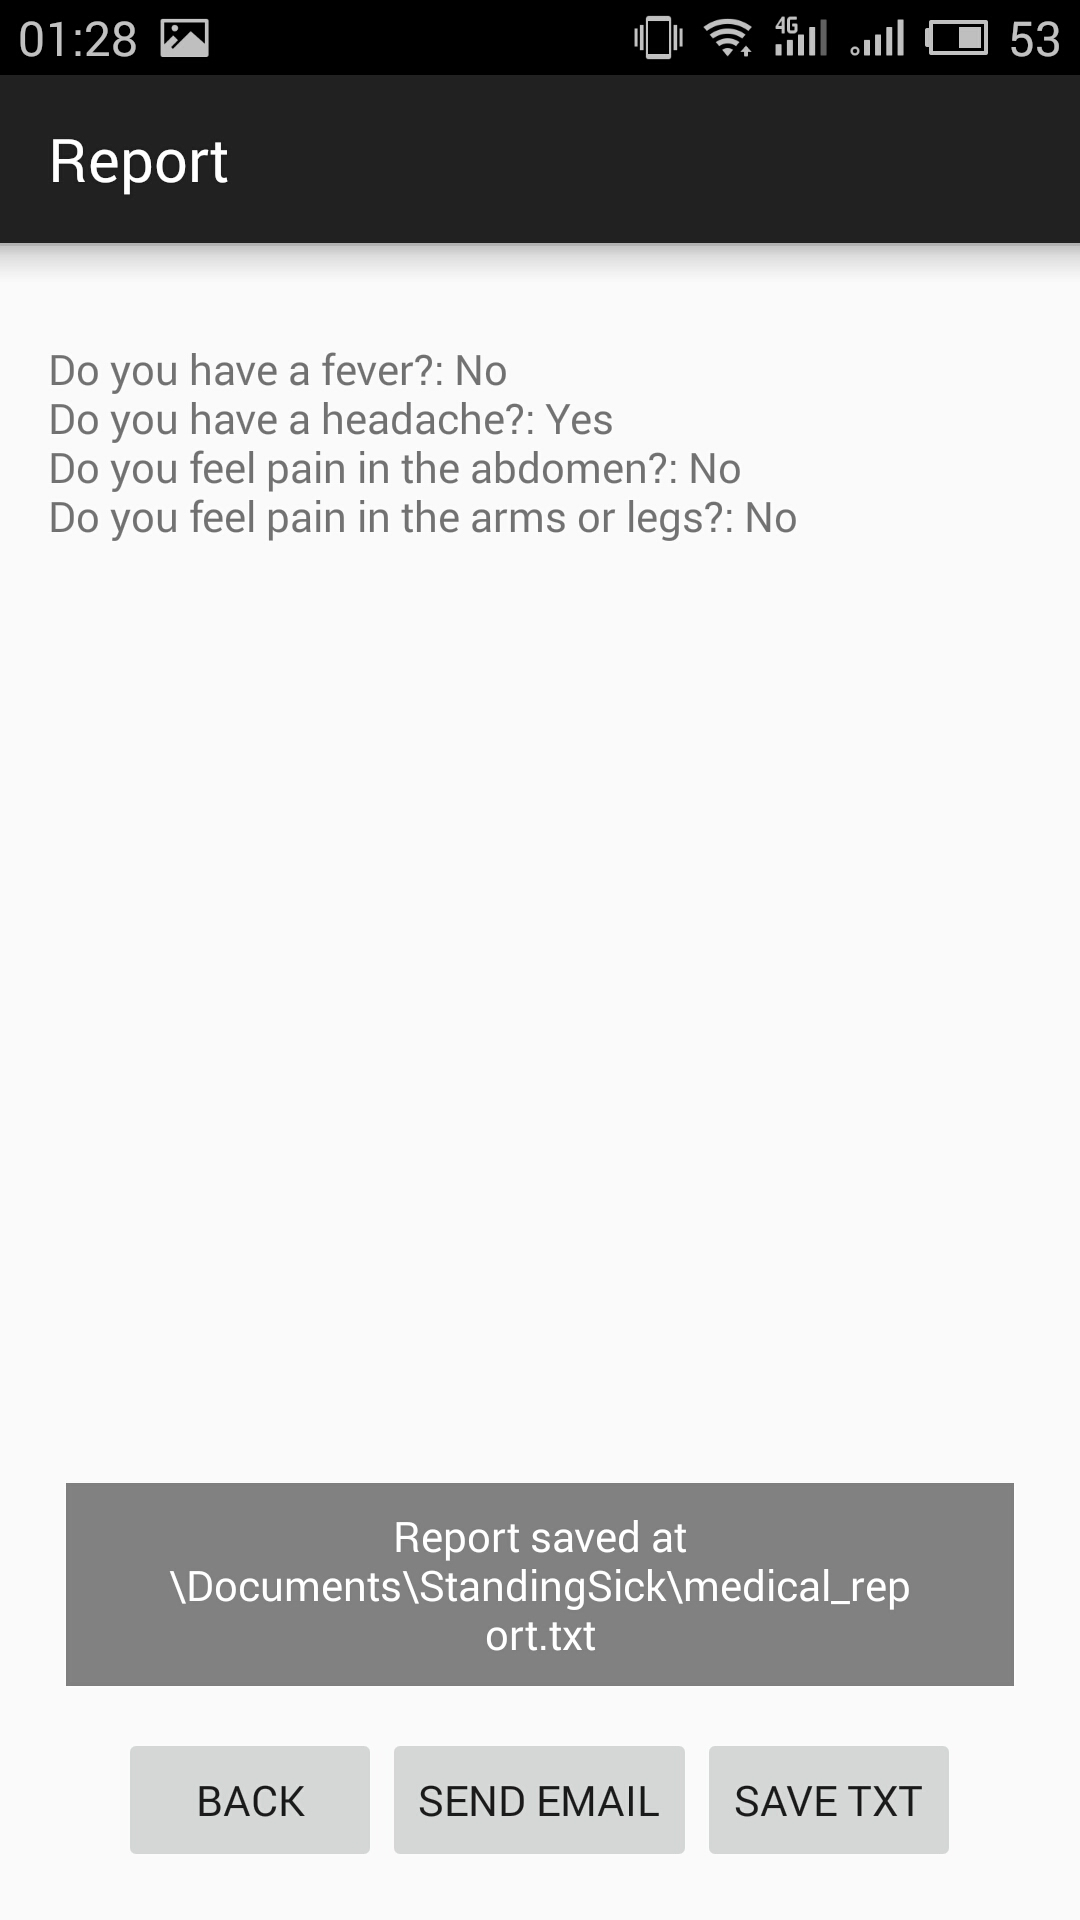
\includegraphics[width=2.0in]{./../img/report.jpg}
  \caption{Report with Toast notification}
  \label{report-ss}
\end{figure}

\begin{figure}[p!]
  \centering
      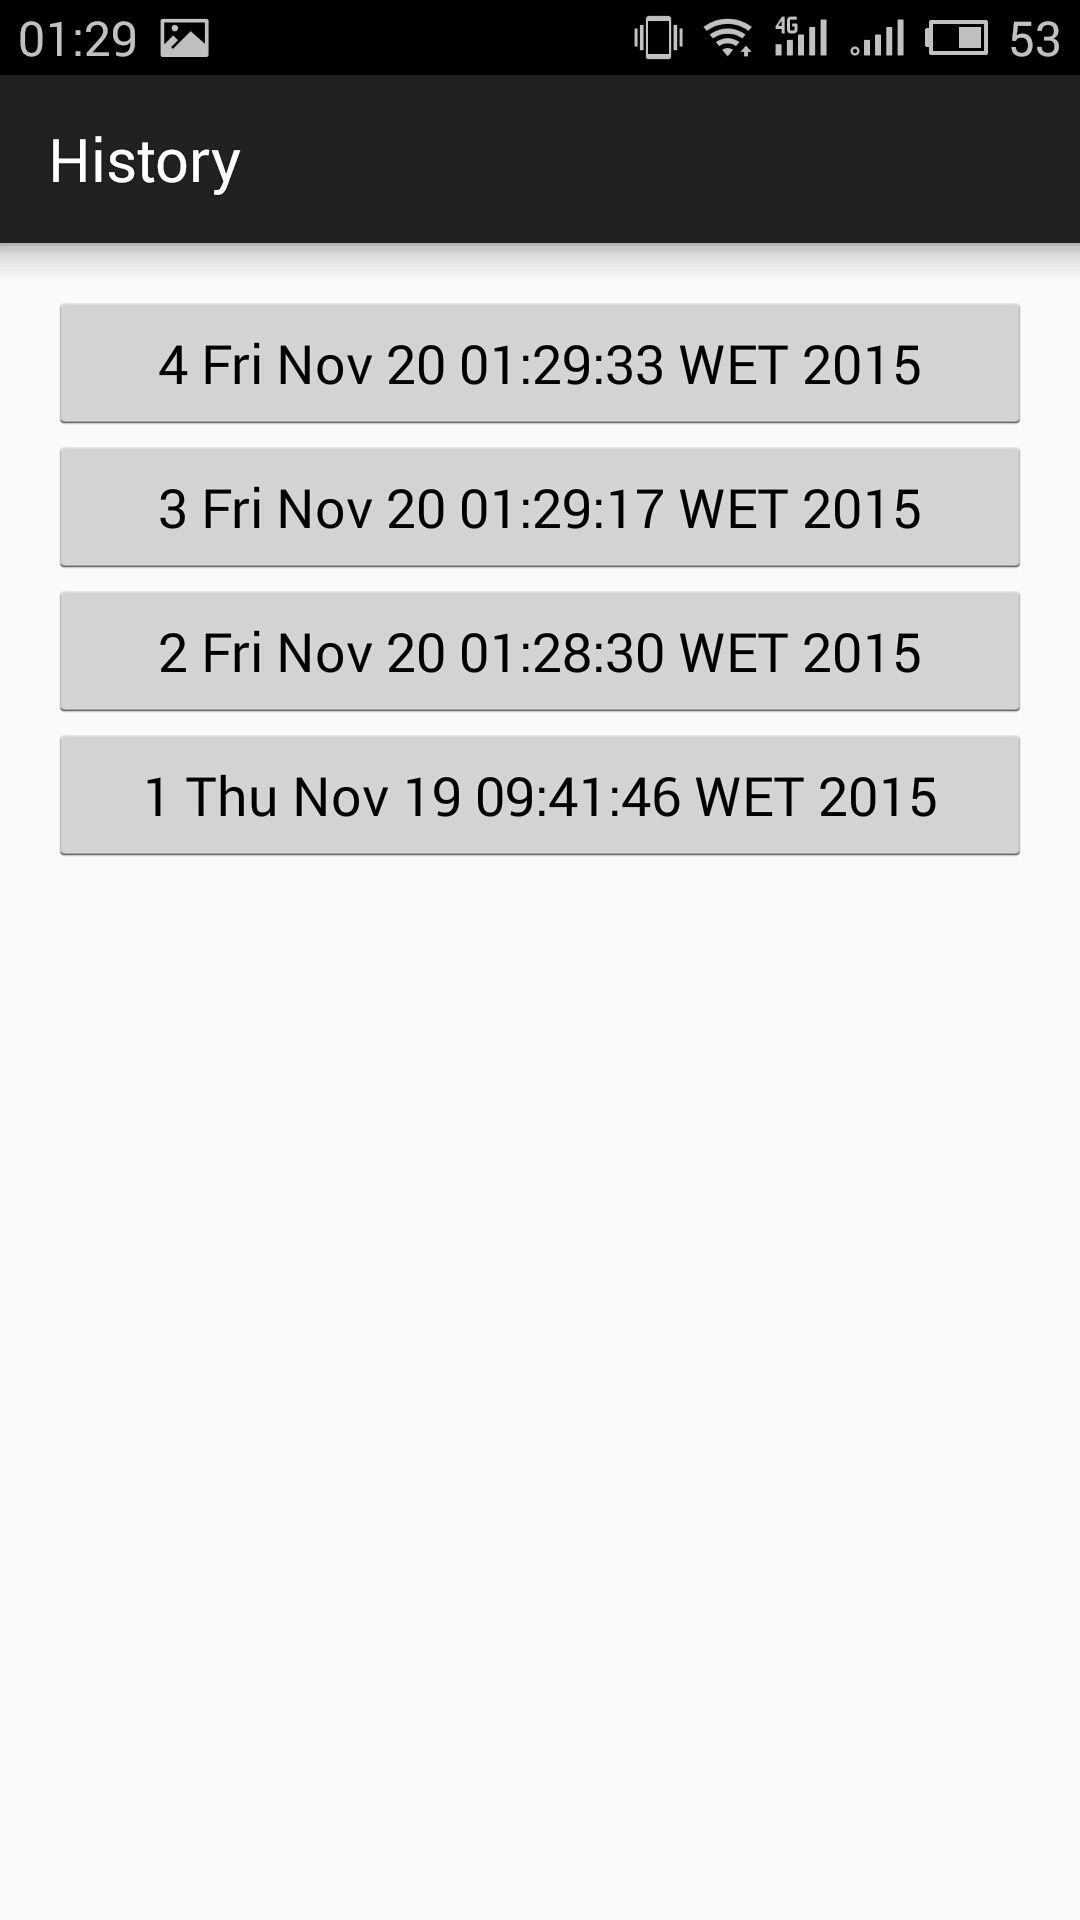
\includegraphics[width=2.0in]{./../img/history.jpg}
  \caption{History Activity}
  \label{history-ss}
\end{figure}

\begin{figure}[p!]
  \centering
      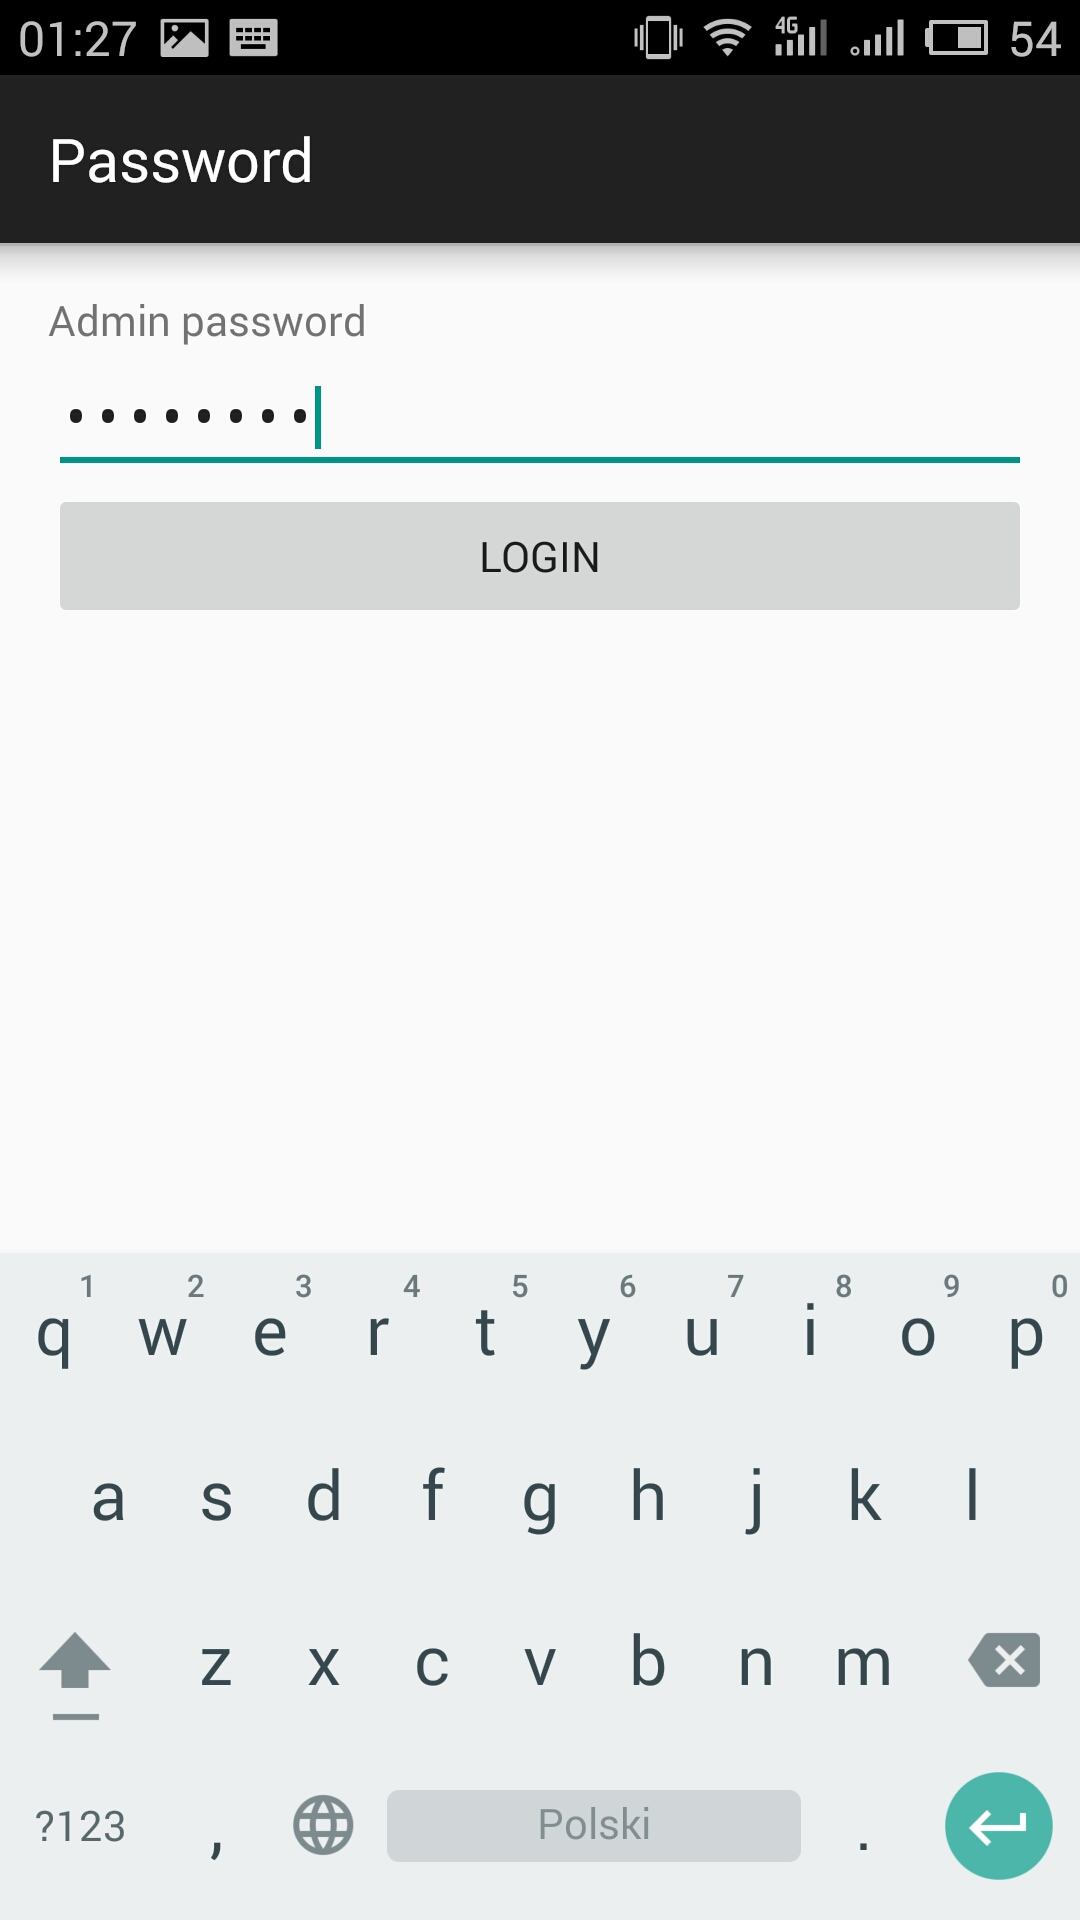
\includegraphics[width=2.0in]{./../img/password.jpg}
  \caption{Password Activity}
  \label{password-ss}
\end{figure}

\begin{figure}[p!]
  \centering
      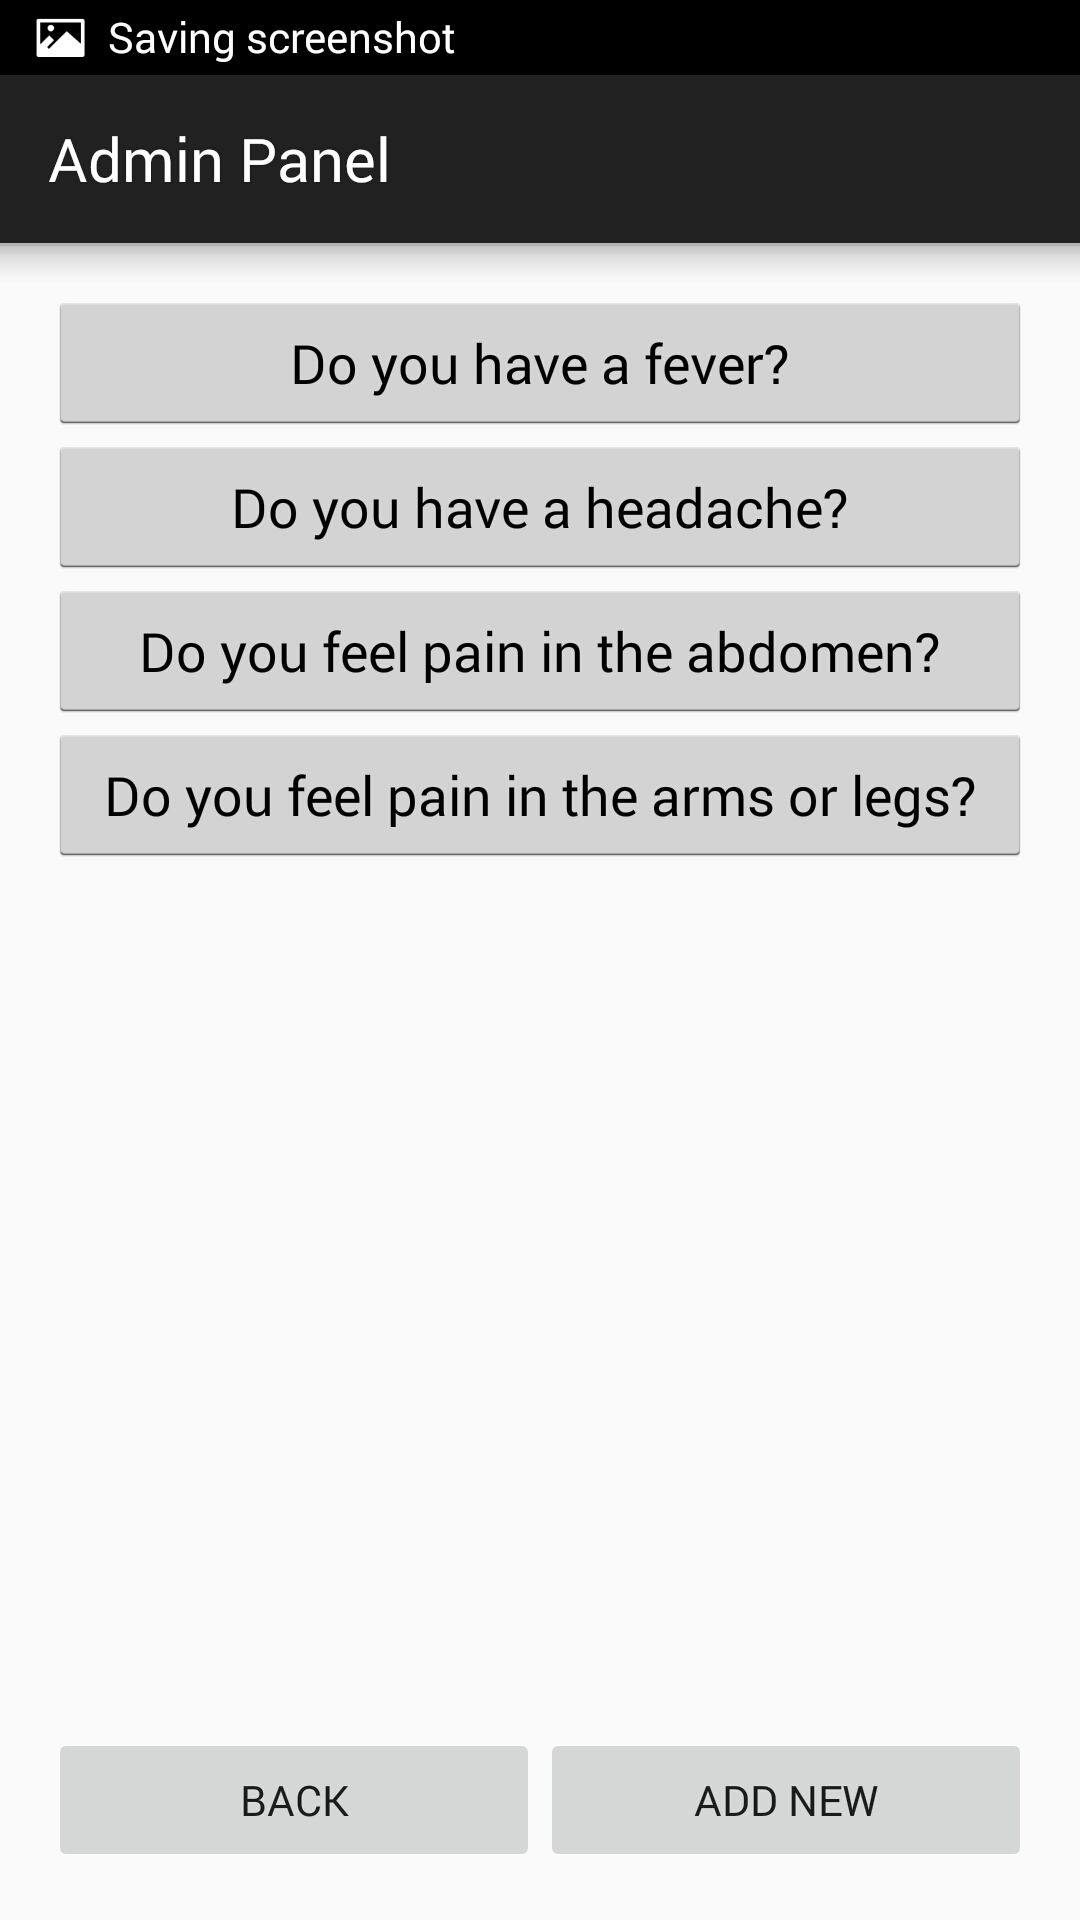
\includegraphics[width=2.0in]{./../img/questions.jpg}
  \caption{Admin Activity}
  \label{questions-ss}
\end{figure}

\begin{figure}[p!]
  \centering
      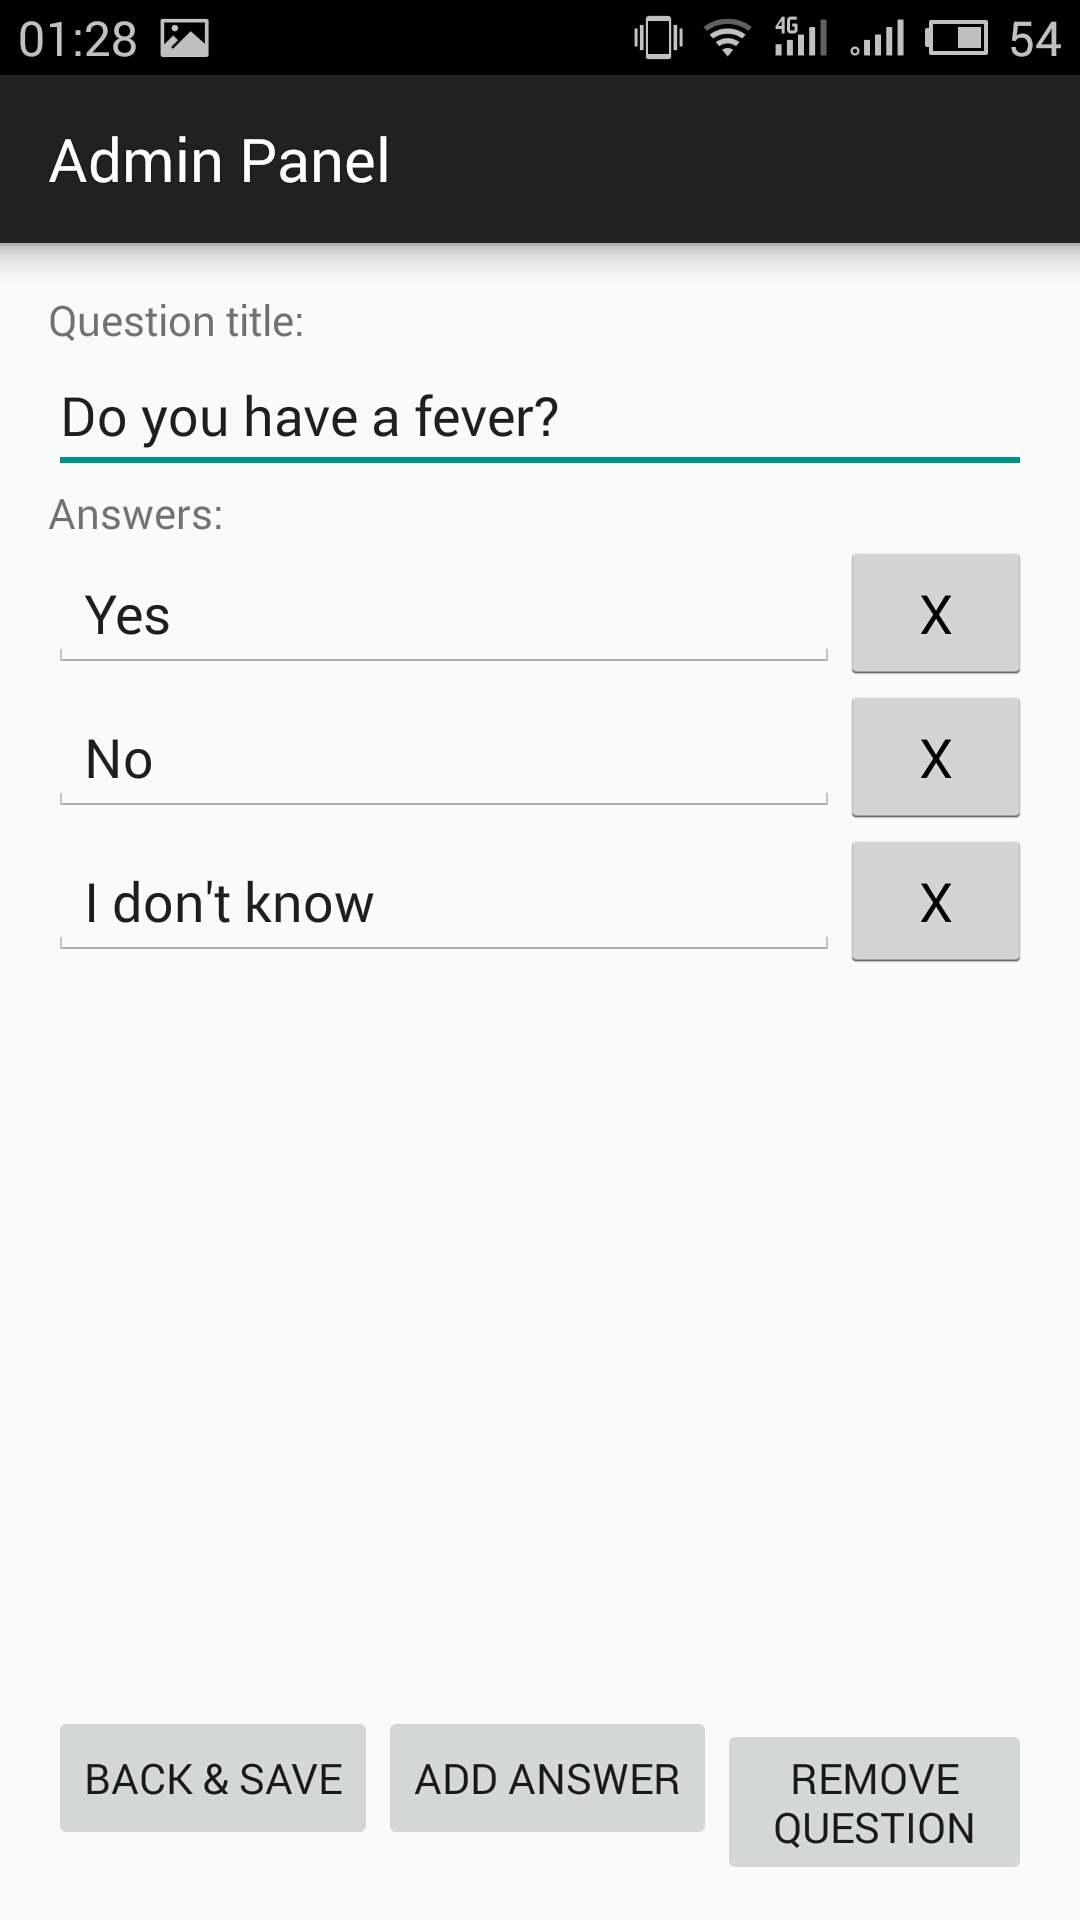
\includegraphics[width=2.0in]{./../img/answers.jpg}
  \caption{Edit Answers}
  \label{answers-ss}
\end{figure}

\clearpage

\begin{lstlisting}[frame=single]
<EditText
  android:layout_width="fill_parent"
  android:layout_height="wrap_content"
  android:password="true"
  android:id="@+id/PasswordEditText"/>
\end{lstlisting}
EditText with anonimized input.\\

\begin{lstlisting}[frame=single]
<ScrollView
  android:layout_width="fill_parent"
  android:layout_height="wrap_content"
  android:layout_weight="1">
  <LinearLayout
    android:layout_width="fill_parent"
    android:layout_height="wrap_content"
    android:orientation="vertical"
    android:id="@+id/AdminAnswersLayout">
  </LinearLayout>
</ScrollView>
\end{lstlisting}
ScrollView for too many answers in admin panel.

\section{Application Implementation}

Section about the details of Implementation. Here are will shown methods how features was made.

\subsection{Environment and Development Technologies}

The project was made in the newest version of Android Studio IDE with the cooperation of version control GIT client - SourceTree. Application was made in pure Android SDK with included SQLite library, no external library was used for this project. 

\subsection{Features Implemented}

\paragraph{SQLite} In every activity who need use data is creating object of class "DatabaseHandle". It is exending class "SQLiteOpenHelper" with specific method to read or write data of database. If it's first run of application, the database is created and filled with example set of questions and answers.

\paragraph{Intents} Intents are used to move between the activities. With intents are sharing some extra data to continue a flow, like: session id in HistoryActivity to ResultActivity or question id from AdminAqtivity to AdminQuestionActivity.

\paragraph{Listeners} Every button has set OnClickListener with onClick method.

\paragraph{Save txt} In ResultActivity is a method "SaveResult()" which is checking if there is available external storage to write, then is make new stream and file is pushed to this stream and saved on external storge. At the end is creating the Toast notification with the state of the operation. Also the application is asking for the acces to write in external storage in AndroidManifest.

\paragraph{Send E-mail} This function is made by calling the specific intent and fill the message with the report.

\paragraph{History} History is made by getting all the sessions from database and dynamically create buttons in LinearLayout. For fit everything on the place was used the ScrollView because there could be more button than can fit on the screen. The same thing was made in editing answers or picking the answer in the poll. In database selected answer is stored by text of question and answer not by connected foreign keys, because if administrator will change the question or remove some answers, in history user still got property data.

\paragraph{Admin Panel} Access to Admin section is protected by the password (admin123). The EditBox got property "password" set to true so the letters are anonymized. In the panel buttons with the questions are create dynamically with from the data. When user push the add new button, then new question is creating and saved in database. During editing the question. The answer EditText boxes with deleting buttons are creating and removing dynamically. Changes in the question or in the answers are saving when your push the back button.

\paragraph{Questions} Activity SurveyActivity are getting the list of a questions with possible answers and replaces it dynamically the view when user click the next button. All anserws radiobuttons are removing and new ones are creating. The buttons got ID the same as the answer id. When there is no more question user are moved to ResultActivity and there is rendering a medical report from the last session.

\subsection{Implementation Details}
In this section will be shown examples of used features of Android API.


\begin{lstlisting}[frame=single]
Toast.makeText(ResultActivity.this,
 "Cannot Save the file",
  Toast.LENGTH_SHORT)
  .show();
\end{lstlisting}
Show this notification when cannot get acces to external storage.\\

\begin{lstlisting}[frame=single]
 public List<Answer> getAnswers(int QId)
    {
SQLiteDatabase db = getReadableDatabase();
List<Answer> answers = 
  =new LinkedList<Answer>();
String[] columns = {"Id", "Content","QId"};
String args[] = {QId+""};
Cursor cursor=db.query("Answers",columns,"
Qid=?",args,null,null,null,null);
while (cursor.moveToNext()){
  Answer answer = new Answer();
  answer.setId(cursor.getLong(0));
  answer.setContent(cursor.getString(1));
  answer.setQId(cursor.getLong(2));
  answers.add(answer);
   }
return answers;
}
\end{lstlisting}
Get Answers for specyfic question.\\

\begin{lstlisting}[frame=single]
LinearLayout ll=(LinearLayout)findViewById
  (R.id.HistoryLayout);
List<Session> sessions = db.getSessions();
final Button[] b = new Button[
sessions.size()];
for(int i=0; i<sessions.size();i++)
{
  b[i]= new Button(this);
ll.addView(b[i]);
b[i].setText(sessions.get(i).getId() 
+ " " + sessions.get(i).getDate());
b[i].setLayoutParams(
  new LinearLayout.LayoutParams(
LinearLayout.LayoutParams.MATCH_PARENT,
LinearLayout.LayoutParams.WRAP_CONTENT));
b[i].setId(sessions.get(i).getId()
  .intValue());
b[i].setOnClickListener(
  new View.OnClickListener() {
  @Override
public void onClick(View v) {
int id =v.getId();
goToResult(id);
            }
        });
        }
\end{lstlisting}
Create buttons in HistoryActivity.\\

\begin{lstlisting}[frame=single]
public void SaveResult()
    {
if(!isExternalStorageWritable())
{
Toast.makeText(ResultActivity.this,
"Cannot Save the file",Toast.LENGTH_SHORT)
.show(); return;
}
File path =
= getFileStorageDir("StandingSick");
File report =
= new File(path,"medical_report.txt");
try {
  FileOutputStream f =
  = new FileOutputStream(report);
  PrintWriter pw = new PrintWriter(f);
  pw.println(content);
  pw.flush();
  pw.close();
  f.close();
  } catch (FileNotFoundException e) {
  e.printStackTrace();
  Toast.makeText(ResultActivity.this,
   "Error",Toast.LENGTH_SHORT).show();
  } catch (IOException e) {
  e.printStackTrace();
  }
Toast.makeText(ResultActivity.this,
"Report saved at \\Documents\\"+
"StandingSick\\medical_report.txt",
Toast.LENGTH_SHORT).show();
    }
\end{lstlisting}
Save the report\\


\begin{lstlisting}[frame=single]
Intent i = new Intent(Intent.ACTION_SEND);
i.setType("message/rfc822");
i.putExtra(Intent.EXTRA_SUBJECT, 
  "medical report");
i.putExtra(Intent.EXTRA_TEXT, content);
try {
  startActivity(Intent.createChooser(i, 
    "Send mail..."));
} catch (android.content.
  ActivityNotFoundException ex) {
Toast.makeText(ResultActivity.this, 
  "There are no email clients installed.",
   Toast.LENGTH_SHORT).show();
}
\end{lstlisting}
Example of sending opening email client by the intent\\

\begin{lstlisting}[frame=single]
Button bb=(Button)
  findViewById(R.id.BackButton);
View.OnClickListener l1 =
= new View.OnClickListener() {
@Override
public void onClick(View v) {
goBack();
}
};
bb.setOnClickListener(l1);
\end{lstlisting}
Example of listener for Back button\\


\section{Conclusion}
Main objectives of this project was achieved. In easy way user can save his time during wait time in queue. Proposition for the update application is work more on design and transform in to material design to better, modern look.





\begin{thebibliography}{1}

\bibitem{SQLlite:Klusiewicz}
Andrzej Klusiewicz, \emph{SQLite in Android Tutorial},\hskip 1em plus
  0.5em minus 0.4em\relax http://andrzejklusiewicz-android.blogspot.pt/2014/02/baza-sqlite-w-androidzie.html
\bibitem{Android}
Google, \emph{Android API GUIDE},\hskip 1em plus
  0.5em minus 0.4em\relax http://developer.android.com/guide/index.html

\end{thebibliography}




% that's all folks
\end{document}


